%
% File acl2016.tex
%
%% Based on the style files for ACL-2015, with some improvements
%%  taken from the NAACL-2016 style
%% Based on the style files for ACL-2014, which were, in turn,
%% Based on the style files for ACL-2013, which were, in turn,
%% Based on the style files for ACL-2012, which were, in turn,
%% based on the style files for ACL-2011, which were, in turn, 
%% based on the style files for ACL-2010, which were, in turn, 
%% based on the style files for ACL-IJCNLP-2009, which were, in turn,
%% based on the style files for EACL-2009 and IJCNLP-2008...

%% Based on the style files for EACL 2006 by 
%%e.agirre@ehu.es or Sergi.Balari@uab.es
%% and that of ACL 08 by Joakim Nivre and Noah Smith

\documentclass[11pt]{article}
\usepackage{acl2016}
\usepackage{times}
\usepackage{url}
\usepackage{latexsym}
\usepackage{graphicx}
\usepackage{amsmath}

%\aclfinalcopy % Uncomment this line for the final submission
%\def\aclpaperid{***} %  Enter the acl Paper ID here

%\setlength\titlebox{5cm}
% You can expand the titlebox if you need extra space
% to show all the authors. Please do not make the titlebox
% smaller than 5cm (the original size); we will check this
% in the camera-ready version and ask you to change it back.

\newcommand\BibTeX{B{\sc ib}\TeX}

\title{Are you asking the right questions? \\ Question generation for filling missing information}

\author{First Author \\
  Affiliation / Address line 1 \\
  Affiliation / Address line 2 \\
  Affiliation / Address line 3 \\
  {\tt email@domain} \\\And
  Second Author \\
  Affiliation / Address line 1 \\
  Affiliation / Address line 2 \\
  Affiliation / Address line 3 \\
  {\tt email@domain} \\}

\date{}

\begin{document}
\maketitle
\begin{abstract}

\end{abstract}
\section{Introduction}

Asking questions is an important aspect of communication. We do not always say everything in detail. According to Gricean pragmatics \cite{}, speakers and listeners adhere to a Cooperative Principle where a speaker communicates information that is as informative as required and not more. This is subjective. Communication is still possible because the listener has the tool of asking questions. By asking questions the listener can elicit information that she thinks is missing. In the field of natural language processing, most previous work on question generation has focused on generating questions whose answers can be found in some aforementioned text. For e.g. generating questions for reading comprehension type of tasks. However there has been little attention paid towards questions that inquire about the missing information in a text. For e.g. consider a post on an online Q \& A forum where a user describes an issue she is facing with an installation on her Ubuntu operating system. A likely question to that post could be \textit{`What version of ubuntu are you using?'}.  Adding the version information could help someone resolve the issue much faster. 

In our work, we ask the following research question: `Can computers learn to ask questions that can help fill in missing information in a given text?'. Asking questions about such missing information is challenging, even for humans. It requires an understanding of what information when added to a given text would increase the utility of the text. When we are trying to teach a computer to ask such questions, an additional challenge is getting the appropriate data to train a machine learning model. In this work, we take a step forward in this direction by making two main contributions:
\begin{enumerate}
\item Introduce a dataset of size X using stackexchange.com that fits our problem scenario
\item Train a model that learns to ask clarifying questions to unanswered posts on stackexchange.com
\end{enumerate}

\begin{figure}[!t]
\centering
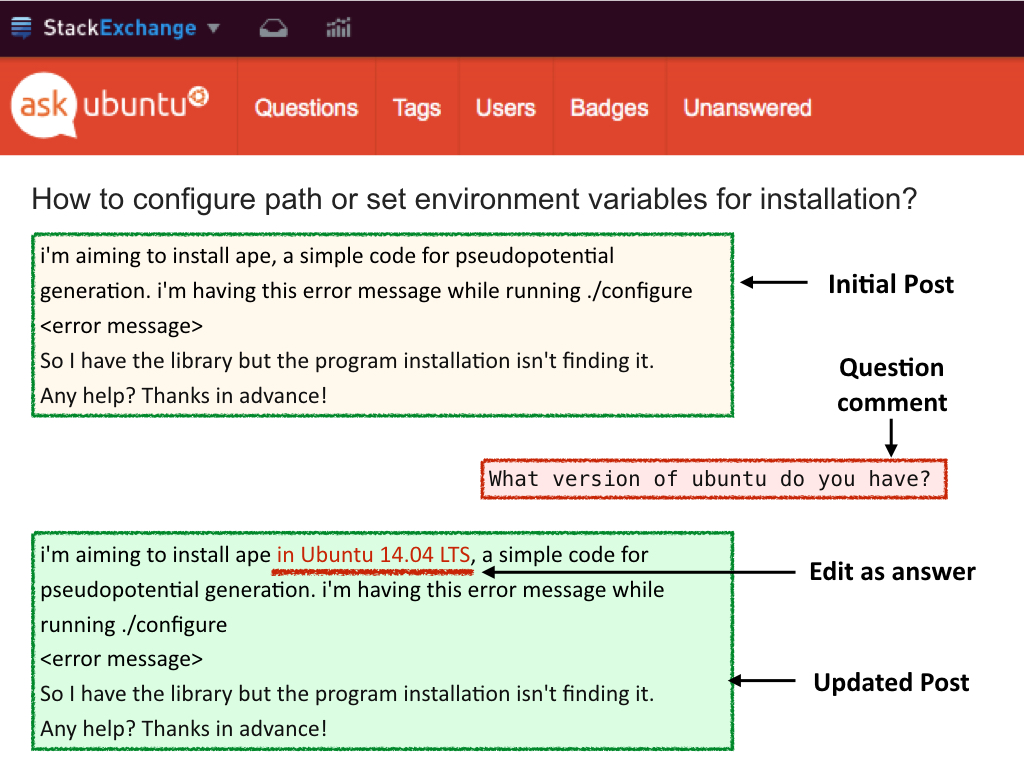
\includegraphics[scale=0.25]{askubuntu_post}
\caption{Example post on askubuntu.com}
\label{askubuntu_post}
\end{figure}

Stackexchange.com is a network of 150+ online question answering communities (including stackoverflow.com, a popular Q\&A forum). Typically, a user posts a question or a concern and other users answer them. However, a lot of these posts remain unanswered. Asaduzzaman et al. \shortcite{asaduzzaman2013answering} say that one of the main reasons for posts remaining unanswered is that they are not clear enough or they are missing some information. Figure 1 shows an example of an unanswered post. These unanswered posts rightly fit our use case of a text with potential missing information that can be filled by asking the right questions. Thus we define our task as given an unanswered post, ask a clarifying question to the post. 

To create our dataset we make the following observation: in several instances, users comment on a given post asking either for some clarification or for some missing information. Subsequently, the author of the post updates the post by adding that piece of missing information. Figure 1 shows an example of such an update. We make use of such updated posts to create our dataset (Section~\ref{dataset}) of \{\textit{post, question, answer}\} triples; where the \textit{post} is the initial post; the \textit{question} is the question comment on the post, and the \textit{answer} is the update made to the post. 

Given a post, we generate question candidates by looking at questions that were asked to posts similar to the given post (Section~\ref{generate_question_candidates}). To identify the most relevant question from the question candidates we take inspiration from an idea in decision theory called the Value of Perfect Information (VPI). VPI measures the worth of gathering additional information. We use this idea in our problem scenario to calculate which question asked to a post when answered would increase the value of the post. We train our model using a neural network framework (described more in Section~\ref{model}) to minimize an objective function defined using VPI. We compare our model with a neural baseline that is trained to select the right question given a post and question candidates; without generating an answer for the question. Human judgements on a held out test set of unanswered posts show that our VPI inspired model can learn to ask questions better.

\iffalse
-- we show that we can train two different models when we have varied amount of training data? (ask Hal)
\fi

\section{Dataset creation}\label{dataset}

Stackexchange.com is a network of online question answering websites about topics in varied fields. The sites are modeled after stackoverflow.com. The data dump of stackexchange.com contains timestamped information about the posts, comments on the post and the history of the revisions made to the post among other things. Our dataset consists of \{\textit{post, question, answer}\} triples: where the \textit{post} is the initial unedited post, the \textit{question} is the comment containing a question and the \textit{answer} is the edit made to the post that matches the question comment. We create the triples from the data dump as follows:
\begin{enumerate}
\item We use the post histories to identify posts that have been updated by its author. We use the timestamp information to retrieve the initial unedited version of a post.
\item Among the several comments made to a post, we extract those that have the question mark `?' token in them. We truncate the comment only till the question mark token to retrieve the question part of the comment.  
\item The final step is to identify the edit made to the post in response to the question comment. Authors make edits to their posts for several reasons; including stylistic updates and grammatical corrections. We use heuristics (Section~\ref{}) to first filter out the edits that have substantial content in them. We then use the timestamp information and a text similarity measure (Section~\ref{}) to match the edits to their respective question comments.
\end{enumerate}

\begin{figure*}[!t]
\centering
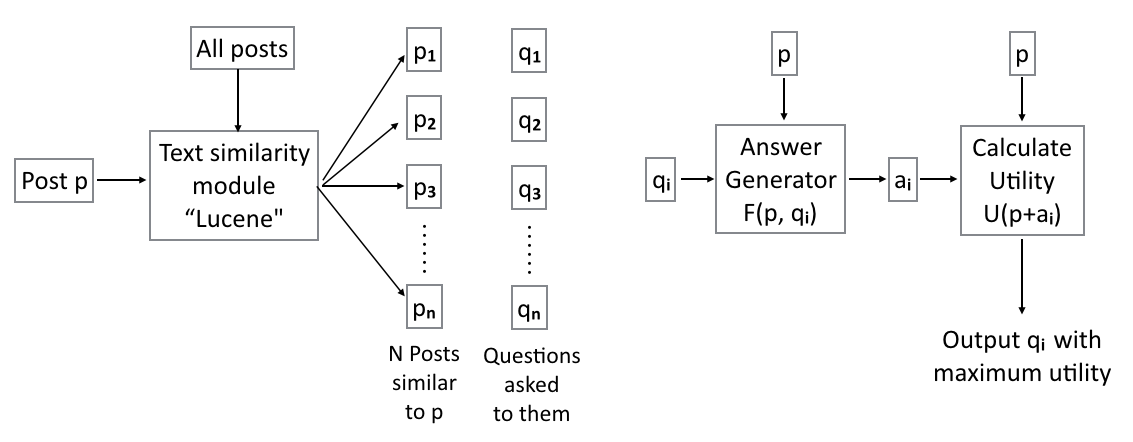
\includegraphics[scale=0.40]{model}
\caption{Three modules of our model: Question candidate generator, Answer generator \& Utility calculator}
\label{model}
\end{figure*}

\section{Model description}\label{model}

Our goal is to develop a model that can learn to ask questions to unanswered posts such that the answers to the questions would add information that is currently missing from the post. We take inspiration from an idea in decision theory called the \textbf{Expected Value of Perfect Information (EVPI)}. Consider a scenario of decision-making aimed at maximizing a certain profit. Suppose we can calculate the expected profit given some information $e$. EVPI measures the worth of collecting additional information $e'$ by calculating the difference between the expected profit given $e$ and the expected profit given $e$ and $e'$. A non-zero value of VPI encourages the collection of the additional information. More formally, EVPI is defined as:\\

$EVPI(e') = EV(e| e') - EV(e)$ \\
where;
\begin{center}
\begin{tabular} {r  l}
$EV$: & Expected Value \\
$e$: & Given information \\
$e'$: & Additional information \\
\end{tabular}
\end{center}

To map this idea to our problem scenario, suppose we have a certain utility of a post. We have to decide whether asking a question to the post is going to increase the utility of the post. There is uncertainty because a question asked to a post can elicit many different answers. Hence we calculate, in expectation, which question among a set of candidate questions will elicit an answer that would maximize the utility of the given post. 

More formally, we train our model using following objective function:\\

$ max_{q \in Q}  E_{a \sim Pr(a|p,q)} U(p+a)$ \\

Given a post $p$, the objective is to select a question $q$ from a set of candidate questions $Q$ such that, an answer $a$ given to the question $q$ would maximize the expected utility of the updated post $U(p+a)$. There are three important pieces to this equation:
\begin{enumerate}
\item Given a post $p$, generate question candidates $Q$ to select a question $q$ from
\item Given a post $p$ and a question $q$, get an answer representation $a$
\item Given an updated post $(p+a)$, calculate the utility of the post 
\end{enumerate}

%During test time, given an unanswered post and a set of candidate questions, we choose the question that maximizes the expected utility of the updated post (once the question is answered). 


\subsection{Generate question candidates}\label{generate_question_candidates}

One way that humans learn to ask questions is by looking at how others ask questions in a similar situation. Using this intuition we generate question candidates for a given post by identifying posts similar to a given post and then looking at the questions asked to those posts. For identifying similar posts, we use Lucene, a software widely used in information retrieval 

We use this intuition to identify potential question candidates for a given post. 
Using the same intuition, Questions asked to posts similar to a given post can be potential question candidates for the given post. 

 We use this algorithm to find the top 20 most similar posts to a given post from the posts in our dataset (Section~\ref{dataset}). We consider the questions asked to these 20 posts as our set of question candidates. 
%- cite regina's work - best matching algorithm (BM25) from information retrieval to get similar posts & hence questions to those posts

\subsection{Generate answer given post and question}

Given a post and a question, there can be several different answers to that question. For e.g. in Figure 1, the question \textit{`Which field are you in?'} can elicit different answers. We therefore want to train a model that learns to generate an answer representation that captures this high-level category of missing information. To train our model we use our dataset of \{\textit{post, question, answer}\} triples (Section~\ref{dataset}). For every post $p_i$, we retrieve 10 similar posts $P_i$ from the dataset using BM25 algorithm (Section~\ref{generate_question_candidates}). During training time, given $\{p_i, q_i, a_i\}$, we use a \textit{post} neural reader, a \textit{question} neural reader and an \textit{answer} neural reader to get their respective neural hidden representations $\{\bar{p_i}, \bar{q_i}, \bar{a_i}\}$.  Given $(\bar{p_i}, \bar{q_i})$, we also define a function $F(\bar{p_i}, \bar{q_i})$ that computes an answer representation from the post and the question. We explain our neural readers and the function $F$ shortly (Section~\ref{neural_readers}). The parameters of all three neural readers and $F$ is learned jointly by minimizing the following objective function:\\

$\sum_i ( {|| F(\bar{p_i}, \bar{q_i}) - \bar{a_i}||}^2 +
 \sum_{j \in P_i} ( {|| F(\bar{p_i, \bar{q_i}}) - \bar{a_j} ||}^2  - {|| \bar{q_i} - \bar{q_j} ||}^2))$\\

The first term forces the function $F$ to generate an answer representation as close as possible to the correct answer $a_i$. The second term exploits the fact that a question can be asked in several different ways. If a question $q_j$ asked to one of the posts $p_j$ similar to post $p_i$ is close to the question $q_i$, then the answer representation generated by function $F$ should also be close to the answer $a_j$ given to the question $q_j$ on the post $p_j$.

\subsection{Calculate utility of a post}

We measure the utility of a post in terms of its completeness. We define the utility function as $U(\bar{p_i}) = [0, 1]$; where a value close to 0 indicates incompleteness and a value close to 1 indicates completeness. To train this model we use a much larger part of the stackexchange.com data dump along with our dataset (Section~\ref{dataset}). We label all the initial unedited posts in our dataset with label 0 and all the updated posts with label 1. Additionally, we label all the unanswered posts in the data dump with label 0 and all the the posts without any question comment in them with label 1. Given a post $p_i$, we use our neural reader (Section~\ref{neural_readers}) to get a post representation $\bar{p_i}$. We train the parameters of our neural reader to minimize the binary cross-entropy between the $sigmoid(\bar{p_i})$ and the label of $p_i$, for all labelled posts. 

\subsection{Our neural reader}\label{neural_readers}

%cite neural readers
The term neural reader is being used increasingly these days to denote a neural network model (like RNN, LSTM, CNN) and its variations (using attention, etc) that is tasked with reading of words in a text and coming up with a representation that helps attain a given goal. Given a sequence of words in a post, a question or an answer, our neural reader uses the long short-term memory architecture (LSTM) \cite{hochreiter1997long} to generate its neural representation. We initialize the word embeddings of each word in our vocabulary using the word2vec \cite{mikolov2013efficient} model trained on the entire data dump of stackexchange.com. We train our neural readers using different objective functions described in previous sections. 

\section{Evaluation method}
%- intrinsic evaluation
% extrinsic evaluation using human judgements

\section{Baseline methods}

\subsection{Bag of words baseline}

\subsection{Neural baseline}

\section{Experiments and Results}\label{experiments_results}

\section{Analysis}

\section{Conclusion}

%In the ongoing effort of making computers better at understanding information, if one were to find something missing, the appropriate question to be asked would be \textit{``How can we make computers better at asking questions? "}

\iffalse

\section{Related Work} \label{related_work}

'Deep Questions without Deep Understanding' 
- generate high-level (they call it deep) question templates by crowdsourcing and then given a text segment, rank question templates that are relevant. 
- We on the other hand make use of existing resources to generate question templates. 

Automatic Factual Question Generation from Text 
- Normal RC type questions generation task
- This is a thesis, so related work section is exhaustive and so can be useful

Automatic Question Generation for Literature Review Writing Support
- Generates questions that can help author write the lit review better
- Input to system is a literature review and o/p is a set of questions
- The system captures all the citations in the paper, extract features out of it and then uses fixed templates to ask questions about the content
- The introduction/motivation of paper is good
						
Generating Natural Questions About an Image 
- Task: Visual Question Generation -- Different from image captioning since the question asked who help infer something from the image that is not directly shown in the image
- Contributions - created new dataset, collected gold annotations and showed that image captioning doesn't do well at this, analyzed several methods and showed deep learning models outperform, created evaluation metric delta-BLEU for this task
			
The Importance of Being Important: Question Generation 
- Why is asking intelligent questions important
- Some related work are relevant

Question Generation from Concept Maps
- Research question - how are questions generated in tutoring systems
- Domain - dialogue between tutor and a student
- They have drawn connections with work in learning/psychology
- Concept map is nothing but a graph with nodes (key terms) and edges (relations like is-a, has-a, etc)
- Their method is to generate concept maps and then have rules to generate questions using these maps
- Highly cited work

Meta Model in Intro to Neuro-Linguistic Programming
- The only answer to the question 'What does a word really mean?' is 'To whom?'
- How do we know we understand someone? By giving their words meaning. Our meaning. Not  their meaning. And there is no guarantee that the two meanings are the same.
- The question we want to explore is, what happens to our thoughts when we clothe them in language, and how faithfully are they preserved when our listeners undress them.
- NLP (Neuro Linguistic Programming) has a very useful map of how language operates called the 'Meta Model'. The Meta Model uses language to clarify language, preventing you from deluding yourself that you understand what words mean; it reconnects language with experience.
- The Meta Model is a series of questions that seek to reverse and unravel the deletions and distortions and generalizations of language. These questions aim to fill in the missing information, reshape the structure and elicit specific information to make sense of the communication.
- Mental map of the speaker
- In an everyday context, the Meta Model gives you a systematic way of gathering information, when you need to know more precisely what a person means. It is a skill that is well worth learning.

Filling Knowledge Gaps in Text for Machine Reading
- In this work they fill the missing gaps with the help of external knowledge bases
- However in our work we suggest that filling the missing information might be hard but asking a question that would point to it is easier and hence more helpful.

Bootstrapping semantic parsing from conversations
- System asks clarification question when asked to parse a sentence 
- Their work is at the sentence level; ours is at discourse level. Also our work is for asking questions about missing information instead of clarification

Work that has used Stackexchange.com data before

\fi
\bibliography{question_generation}
\bibliographystyle{acl2016}


\end{document}
